\section{Proceso B\'asico del Reconocimiento del Habla}

\begin{frame}{Proceso B\'asico del Reconocimiento del Habla (1/12)}
\uncover<1-2>{
\begin{quote}
\emph{La b\'usqueda de la oraci\'on m\'as probable W perteneciente al lenguaje L, dada la entrada ac\'ustica 0.}
\end{quote}
}

\uncover<2-2>{
\begin{align}
\hat{W} = \argmax_{W \in L} \overbrace{P(O|W)}^\text{M. ac\'ustico}\overbrace{P(W)}^\text{M. de lenguaje}
\label{eq:asrFundamental}
\end{align}
}
\end{frame}

\begin{frame}{Proceso B\'asico del Reconocimiento del Habla (2/12)}

\begin{figure}[H] 
\centering
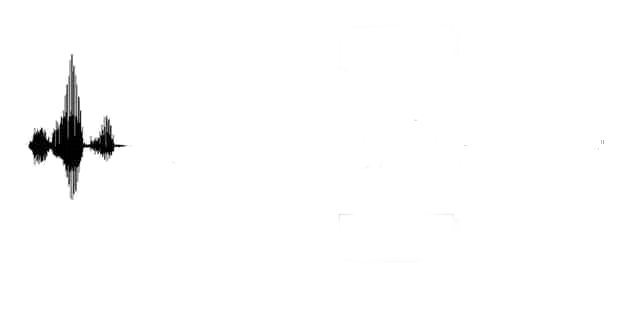
\includegraphics[width=0.8\textwidth]{./graphics/proceso_00.png}
\caption{Proceso del reconocimiento del habla.}
\label{figure:proceso}
\end{figure}
\end{frame}

\begin{frame}{Proceso B\'asico del Reconocimiento del Habla (2/12)}

\begin{figure}[H] 
\centering
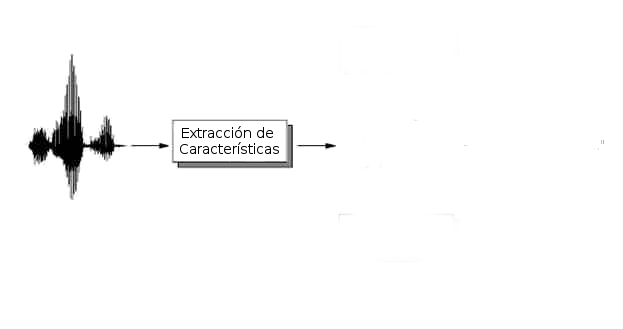
\includegraphics[width=0.8\textwidth]{./graphics/proceso_0.png}
\caption{Proceso del reconocimiento del habla.}
\label{figure:proceso}
\end{figure}
\end{frame}

\begin{frame}{Proceso B\'asico del Reconocimiento del Habla (2/12)}

\begin{figure}[H]  
\centering
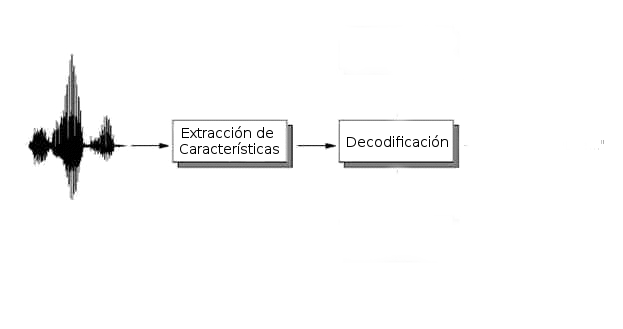
\includegraphics[width=0.8\textwidth]{./graphics/proceso_1.png}
\caption{Proceso del reconocimiento del habla.}
\label{figure:proceso}
\end{figure}
\end{frame}

\begin{frame}{Proceso B\'asico del Reconocimiento del Habla (2/12)}

\begin{figure}[H] 
\centering
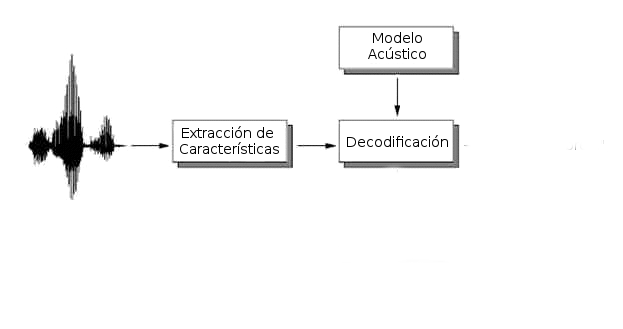
\includegraphics[width=0.8\textwidth]{./graphics/proceso_2.png}
\caption{Proceso del reconocimiento del habla.}
\label{figure:proceso}
\end{figure}
\end{frame}

\begin{frame}{Proceso B\'asico del Reconocimiento del Habla (2/12)}

\begin{figure}[H] 
\centering
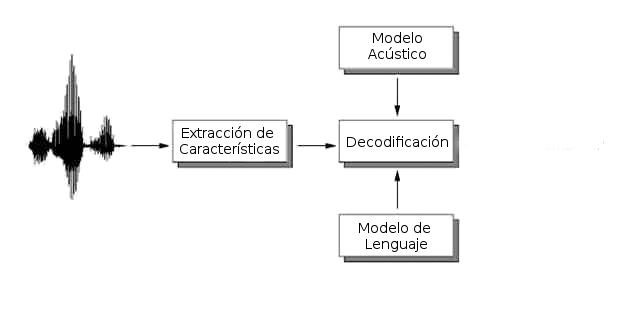
\includegraphics[width=0.8\textwidth]{./graphics/proceso_3.png}
\caption{Proceso del reconocimiento del habla.}
\label{figure:proceso}
\end{figure}
\end{frame}

\begin{frame}{Proceso B\'asico del Reconocimiento del Habla (2/12)}

\begin{figure}[H] 
\centering
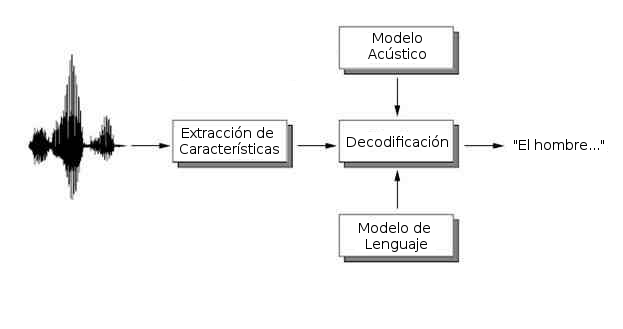
\includegraphics[width=0.8\textwidth]{./graphics/proceso.png}
\caption{Proceso del reconocimiento del habla.}
\label{figure:proceso}
\end{figure}
\end{frame}


\begin{frame}{Proceso B\'asico del Reconocimiento del Habla (3/12)}
\framesubtitle{Fase 1: Extracci\'on de caracter{\'\i}sticas}
\begin{figure}[H]
\centering
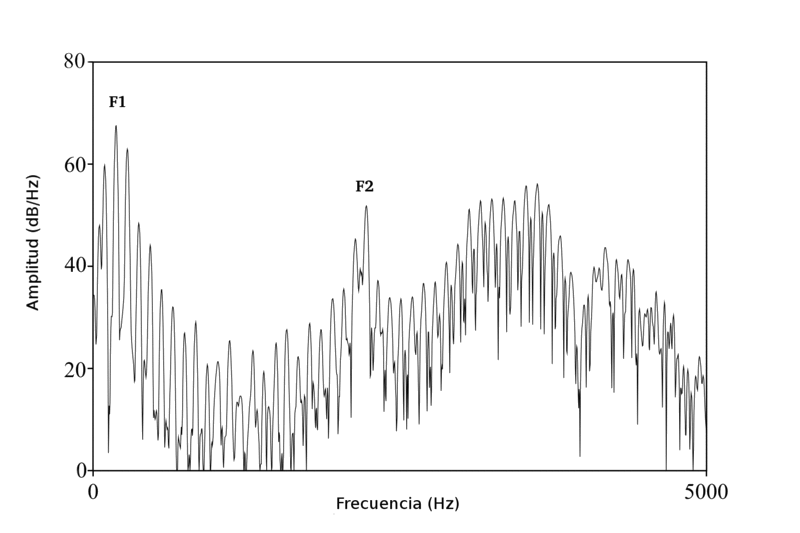
\includegraphics[width=0.9\linewidth]{./graphics/formantes.png}
\caption{Representaci\'on del espectro en el cual pueden identificarse los picos espectrales o formantes.}
\label{figure:formants}
\end{figure}
\end{frame}

\begin{frame}{Proceso B\'asico del Reconocimiento del Habla (4/12)}

\begin{figure}[H]
\centering
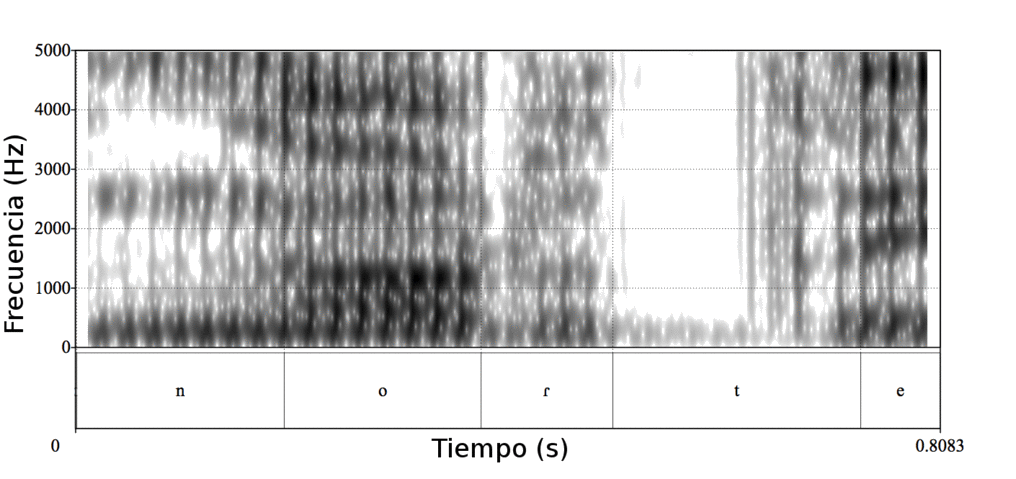
\includegraphics[width=1\linewidth]{./graphics/espectrograma.png}
\caption{Representaci\'on de un espectrograma, puede verse como una colecci\'on de espectros  ubicados uno despu\'es de otro.}
\label{figure:spectrogram}
\end{figure}

\end{frame}

\begin{frame}{Proceso B\'asico del Reconocimiento del Habla (5/12)}
\framesubtitle{Fase 1: Extracci\'on de caracter{\'\i}sticas}

\begin{figure}[H] 
\centering
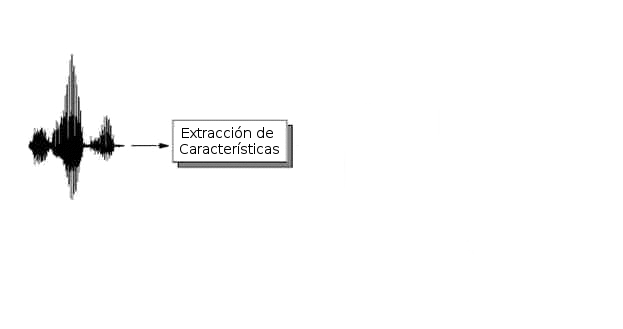
\includegraphics[width=0.8\textwidth]{./graphics/extraccion_0.png}
\caption{Fase de extracci\'on de caracter{\'\i}sticas.}
\label{figure:hmm}
\end{figure}
\end{frame}

\begin{frame}{Proceso B\'asico del Reconocimiento del Habla (5/12)}
\framesubtitle{Fase 1: Extracci\'on de caracter{\'\i}sticas}

\begin{figure}[H] 
\centering
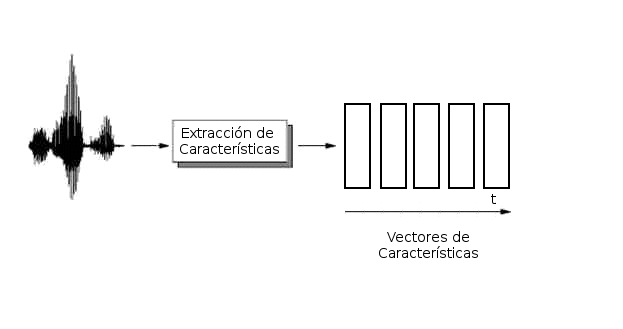
\includegraphics[width=0.8\textwidth]{./graphics/extraccion.png}
\caption{Fase de extracci\'on de caracter{\'\i}sticas.}
\label{figure:hmm}
\end{figure}
\end{frame}


\begin{frame}{Proceso B\'asico del Reconocimiento del Habla (6/12)}
\framesubtitle{Fase 2: Decodificaci\'on: Modelo de Lenguaje}
\uncover<1-3>{Probabilidad de ocurrencia de una secuencia de palabras $x_1,x_2,\ldots,x_n$ para un lenguaje dado.}
\vspace*{2\baselineskip}
\begin{itemize}
    \uncover<2-3>{\item Basado en N-Gramas
        \small \begin{equation*}
            \hspace*{-1.5cm} 
            p(\text{el, hombre, corre}) = p(el \mid \text{\textless} s\text{\textgreater}) \, 
            p(\text{\emph{hombre}} \mid el) \, p(corre \mid \text{\emph{hombre}}) \, 
            p(\text{\textless} /s\text{\textgreater} \mid corre)
        \end{equation*}}
        \vspace*{1\baselineskip}
        \uncover<3-3>{\item Basado en Gram\'atica
        \begin{bnf*}
            \bnfprod{pregunta}
            {\bnfts{Cu\'al} \bnfsp \bnfts{es} \bnfsp \bnfts{la}  \bnfpn{info} \bnfsp  \bnfts{en} \bnfsp \bnfpn{ciudad}} \\
            \bnfprod{info}
            {\bnfts{temperatura} \bnfor \bnfts{presi\'on atmosf\'erica} \bnfor \bnfts{hora}} \\
            \bnfprod{ciudad}
            {\bnfts{Par{\'\i}s} \bnfor \bnfts{Nueva York} \bnfor \bnfts{Roma}}
        \end{bnf*}}
    \end{itemize}
\end{frame}

\begin{frame}{Proceso B\'asico del Reconocimiento del Habla (7/12)}
\framesubtitle{Fase 2: Decodificaci\'on - Modelo Ac\'ustico}

\setbeamercovered{transparent}
\uncover<1-9>{Probabilidad de una entrada ac\'ustica $O$ dada una secuencia de \mbox{palabras $W$.}}
\begin{columns}
\column{0.45\linewidth}
\visible<2-9>{
\begin{itemize}
    \uncover<1-9>{\item Modelos Ocultos de Markov}
        \begin{itemize}
                \uncover<4-9>{\item Estados: $S$}
                \uncover<5-9>{\item Observaciones: $V$}
                \uncover<6-9>{\item Probabilidad inicial: $\pi$}
                \uncover<7-9>{\item Probabilidad de transici\'on: $a$}
                \uncover<8-9>{\item Probabilidad de observaci\'on: $b$}
        \end{itemize}
    \uncover<9-9>{\item Diccionario Fon\'etico}
\end{itemize}
}

\column{0.55\linewidth}
\begin{figure}[H]
\centering
\uncover<3-9>{
\visible<3-9>{
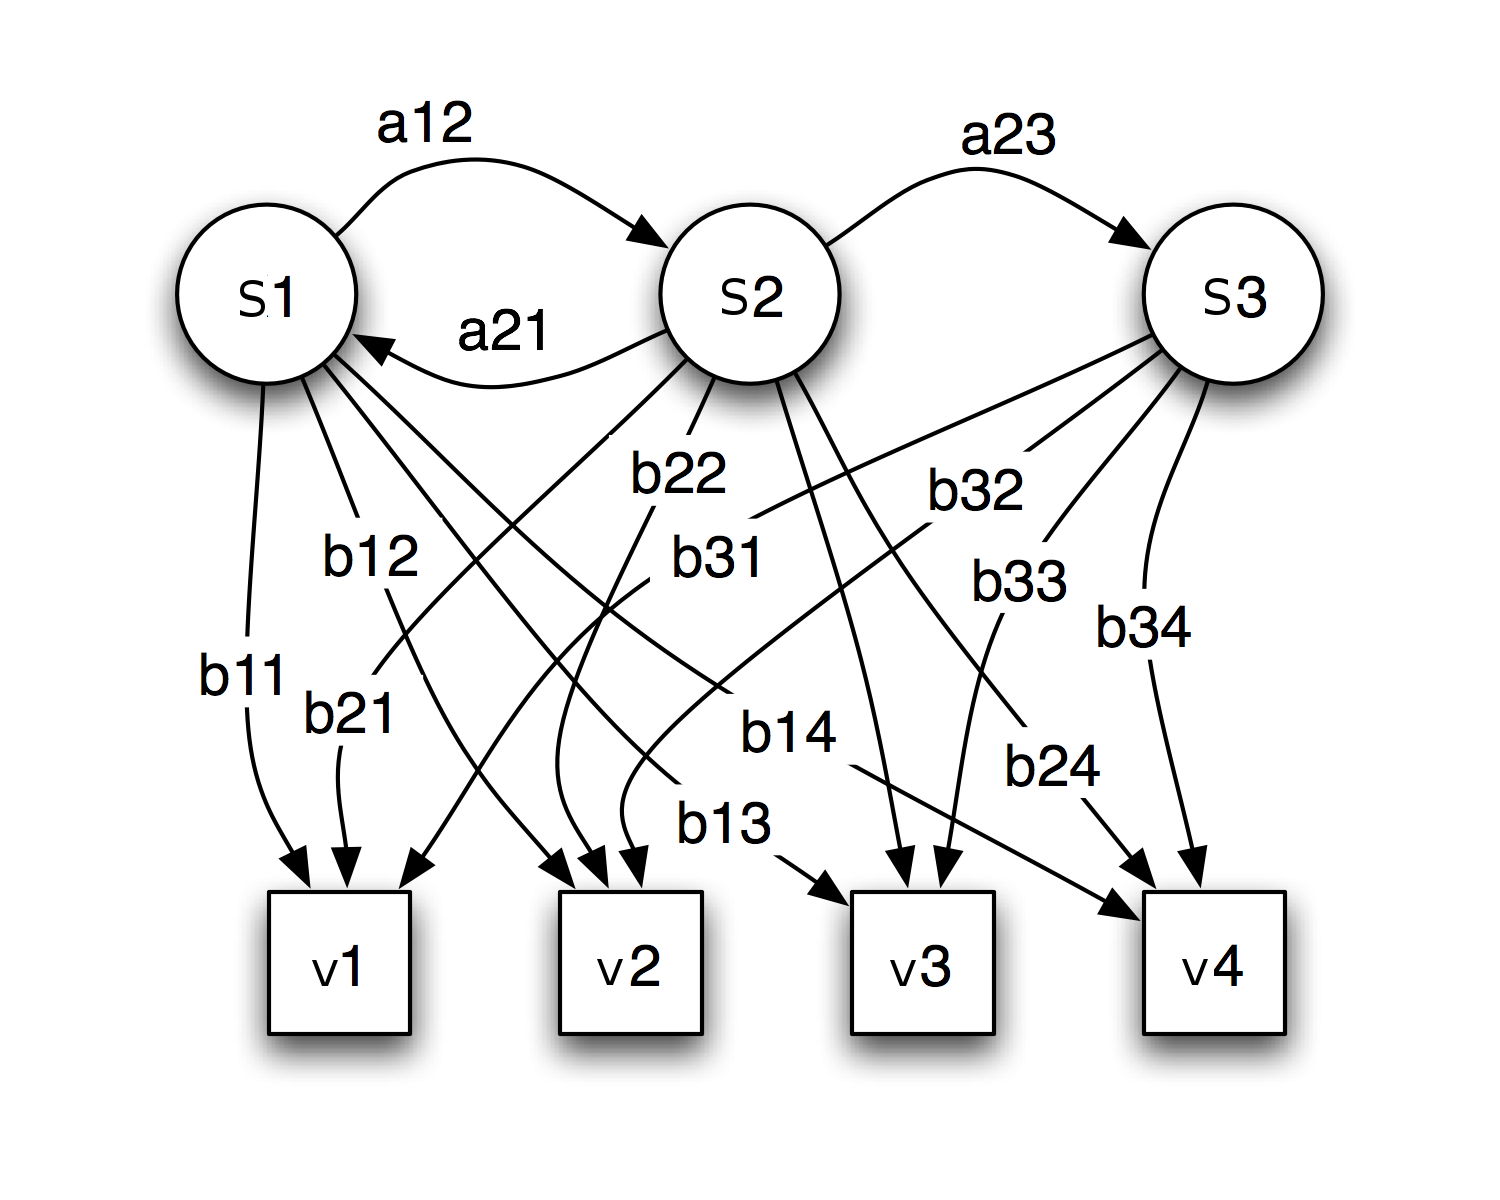
\includegraphics[width=1\textwidth]{./graphics/hmm.png}
\caption{Representaci\'on de un modelo oculto de Markov.}}}
\label{figure:esquema-herramientas}
\end{figure}
\end{columns}


\end{frame}

\begin{frame}{Proceso B\'asico del Reconocimiento del Habla (8/12)}
\framesubtitle{Un ejemplo sencillo}
\uncover<1-2>{
\begin{table}[H]
\centering
\footnotesize
\begin{tabular}{|p{1.5cm}|p{1.5cm}|p{1.5cm}|p{1.5cm}|p{1.5cm}|}
\hline
P(.,.)  &   la & casa & roja & Final\texttt{\_}frase \\
\hline
Inicio\texttt{\_}frase & 0.8 & 0 & 0.2 & 0 \\
 \cline{1-1}
la  &  0 & 0.7 & 0.3 & 0   \\
 \cline{1-1}
casa & 0 & 0 & 0.75 & 0.25 \\
 \cline{1-1}
roja  & 0 & 0 & 0 & 1     \\
\hline  
\end{tabular}
\label{sec:tabla-ejemplo1}
\end{table}
}

\uncover<2-2>{
\begin{figure}[H] 
\centering
\visible<2-2>{
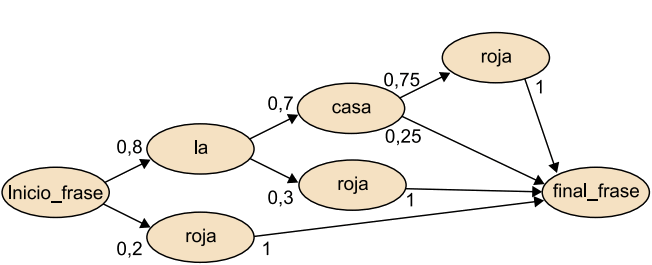
\includegraphics[width=0.8\textwidth]{./graphics/ejemplo1.png}
\caption{Espacio de Búsqueda simplificado.}}
\label{figure:ejemplo1}
\end{figure}
}

\end{frame}

\begin{frame}{Proceso B\'asico del Reconocimiento del Habla (9/12)}
\framesubtitle{Un ejemplo sencillo}
\uncover<1-4>{
\begin{figure}[H] 
\centering
\visible<1-4>{
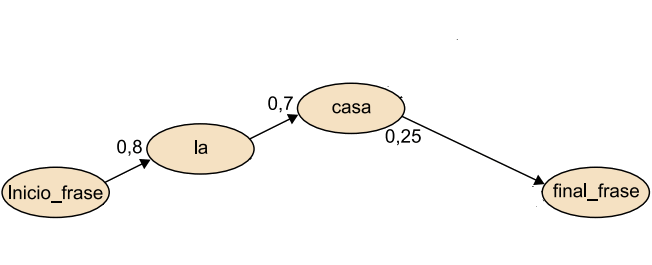
\includegraphics[width=0.8\textwidth]{./graphics/ejemplo2.png}
\caption{Un camino de búsqueda posible.}}
\label{figure:ejemplo2}
\end{figure}
}

\begin{equation*}
\begin{split}
\uncover<2-4>{P(W) & = P(la |(<Inicio\texttt{\_}frase>) P(casa|la)P(<Final\texttt{\_}frase>| casa)} \\
\uncover<3-4>{& = 0,8 \times 0,7 \times 0,25} \\
\uncover<4-4>{& = 0,14}
\end{split}
\end{equation*}

\end{frame}


\begin{frame}{Proceso B\'asico del Reconocimiento del Habla (10/12)}
\framesubtitle{Un ejemplo sencillo}

\uncover<1-2>{

``la casa'' $\rightarrow$ $[$ $l\!\!+\!\!a$\quad $\underbrace{l\!\!-\!\!a\!\!+\!\!k}$\quad $a\!\!-\!\!k\!\!+\!\!a$\quad $k\!\!-\!\!a+\!\!s$\quad $a\!\!-\!\!s\!\!+\!\!a$\quad $s\!\!-\!\!a$ $]$
}



\begin{figure}[H] 
\centering
\visible<2-2>{
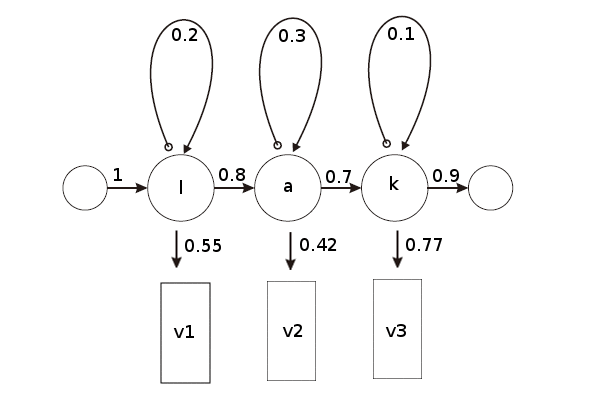
\includegraphics[width=0.6\textwidth]{./graphics/ejemplo3.png}
\caption{Modelo oculto de Markov para $l\!\!-\!\!a\!\!+\!\!k$.}}
\label{figure:ejemplo3}
\end{figure}


\end{frame}

\begin{frame}{Proceso B\'asico del Reconocimiento del Habla (11/12)}
\framesubtitle{Un ejemplo sencillo}


\begin{figure}[H] 
\centering
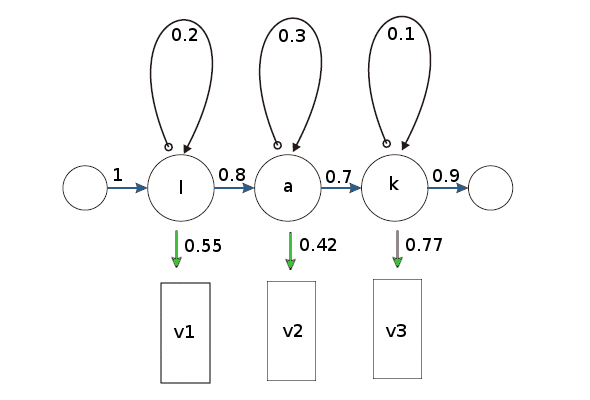
\includegraphics[width=0.6\textwidth]{./graphics/ejemplo4.png}
\caption{Probabilidad de un camino posible para $l\!\!-\!\!a\!\!+\!\!k$.}
\label{figure:ejemplo4}
\end{figure}

\begin{equation*}
\begin{split}
\uncover<2-3>{P(O|W) & = 1 \times 0,55 \times 0,8 \times 0,42 \times 0,7 \times 0,77 \times 0.9} \\
\uncover<3-3>{& = 0,089}
\end{split}
\end{equation*}


\end{frame}


\begin{frame}{Proceso B\'asico del Reconocimiento del Habla (12/12)}
\framesubtitle{Un ejemplo sencillo}

\uncover<1-5>{
``la casa'' $\rightarrow$ $[$ $\underbrace{l\!\!+\!\!a}_{0,47}$\quad $\underbrace{l\!\!-\!\!a\!\!+\!\!k}_{0,089}$\quad $\underbrace{a\!\!-\!\!k\!\!+\!\!a}_{0,34}$\quad $\underbrace{k\!\!-\!\!a+\!\!s}_{0,33}$\quad $\underbrace{a\!\!-\!\!s\!\!+\!\!a}_{0,22}$\quad $\underbrace{s\!\!-\!\!a}_{0,44}$ $]$
}

\begin{equation*}
\begin{split}
\uncover<2-5>{P(O|W) & = 0,47 \times 0,089 \times 0,34 \times 0,33 \times 0,22 \times 0,44 } \\
\uncover<3-5>{ & = 0,00045} \\
\uncover<4-5>{P(O|W) P(W) & = 0,00045 \times 0,14 } \\
\uncover<5-5>{& = 6.36\e{-5}}
\end{split}
\end{equation*}

\end{frame}

% \begin{frame}{Proceso B\'asico del Reconocimiento del Habla (7/8)}
% \framesubtitle{Fase 2: Decodificaci\'on - B\'usqueda}

% \setbeamercovered{transparent}
% \begin{columns}
% \column{0.30\linewidth}
% \visible<1-3>{
% \begin{itemize}
%     \uncover<2-3>{\item Algoritmo de Viterbi.}
%     \uncover<3-3>{\item Algoritmo A*.}
% \end{itemize}
% }

% \column{0.7\linewidth}
% \begin{figure}[H]
% \centering
% \uncover<1-3>{
% 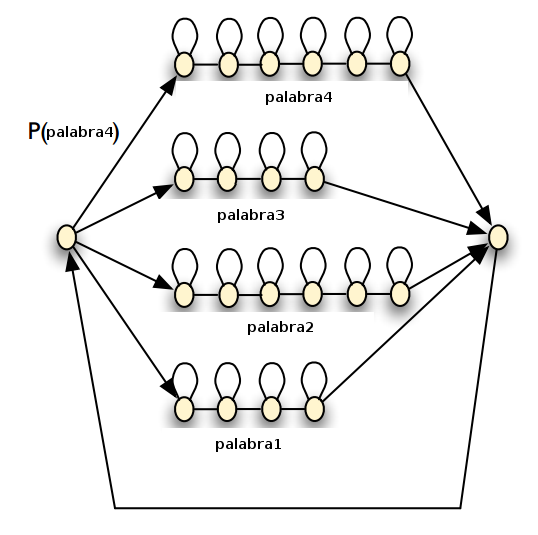
\includegraphics[width=0.8\textwidth]{./graphics/espacio.png}
% \caption{Espacio de b\'usqueda para un lenguaje simple de cuatro palabras. Traducido a partir de \cite{RenalsSearch}.}}
% \label{figure:espacio-busqueda}
% \end{figure}
% \end{columns}


% \end{frame}

% \begin{frame}{Proceso B\'asico del Reconocimiento del Habla (8/8)}
% \framesubtitle{Fase 2: Decodificaci\'on}
% \begin{figure}[H] 
% \centering
% 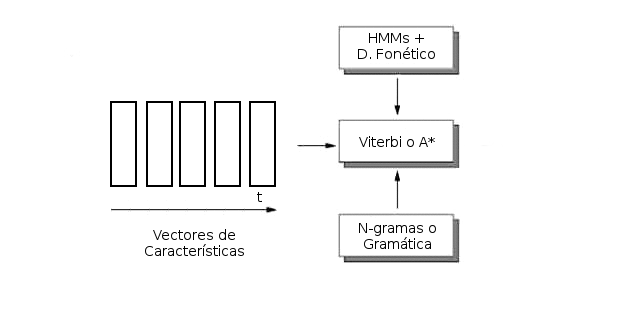
\includegraphics[width=0.8\textwidth]{./graphics/decodificacion0.png}
% \caption{Fase de decodificaci\'on.}
% \label{figure:decoding}
% \end{figure}
% \end{frame}


% \begin{frame}{Proceso B\'asico del Reconocimiento del Habla (8/8)}
% \framesubtitle{Fase 2: Decodificaci\'on}
% \begin{figure}[H] 
% \centering
% 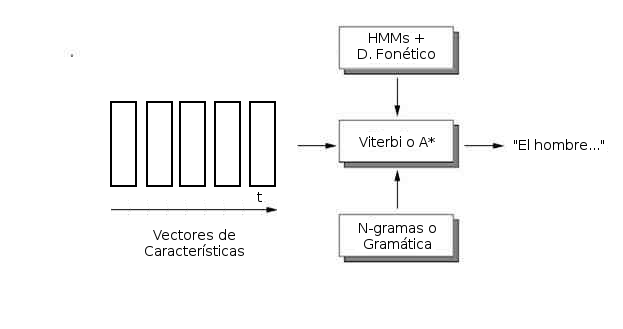
\includegraphics[width=0.8\textwidth]{./graphics/decodificacion.png}
% \caption{Fase de decodificaci\'on.}
% \label{figure:decoding}
% \end{figure}
% \end{frame}
